\section{Auswertung}
\subsection{Statische Methode}
Die gemessenen Temperaturen für die vom Peltier-Element fernen Thermoelemente werden in der Abbildung 2 dargestellt.
Es wird die Temperatur der fernen Thermoelemente für Messing, Aluminium und Edelstahl gegen die Zeit aufgetragen.
Dabei wird einmal die schmale und die breite Platine Messing verwendet.
\begin{figure}[H]
    \centering
    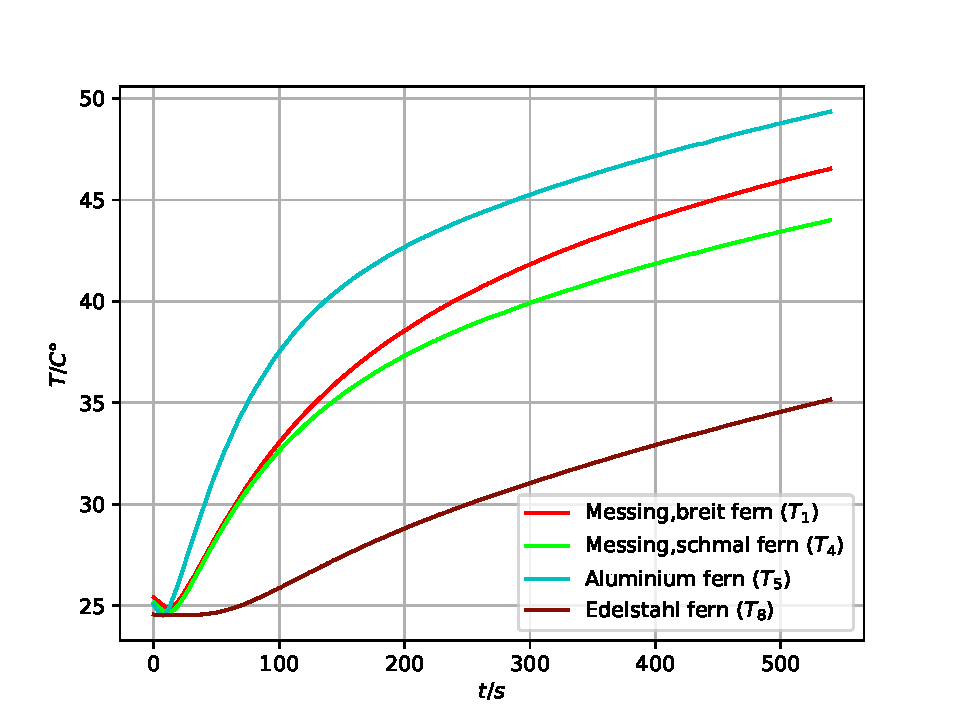
\includegraphics{Statisch.pdf}
    \caption{Temperaturverläufe der Thermoelemente 1,4,5 und 8.}
    \label{fig:a}
\end{figure}

Die einzelnen Thermoelemente erreichen folgende Höchstwerte nach $\SI{540}{s}$.

\begin{equation}
    T1 = \SI{46,53}{°C} \notag
\end{equation}
\begin{equation}
    T4 = \SI{43,99}{°C} \notag
\end{equation}
\begin{equation}
    T5 = \SI{49,35}{°C} \notag
\end{equation}
\begin{equation}
    T8 = \SI{35,15}{°C} \notag
\end{equation}

Es lässt sich sagen, dass alle Kurven ein exponentielles Wachstum haben, welches sich für jeden Stoff gegen eine andere Maximaltemperatur nähert.
Dabei erreicht das Thermoelement aus Aluminium die höchste Temperatur und hat somit die beste Wärmeleitfähigkeit $\kappa$, während Edelstahl die geringste Temperatur erreicht.
Bei den beiden Thermoelementen aus Messing, erreicht das breitere Thermoelement die höhere Temperatur aufgrund der größeren Querschnittsfläche.

Aus Gleichung (1) lässt sich der Wärmestrom folgendermaßen bestimmen.
\begin{equation}
    \frac{\Delta Q}{\Delta t} = -\kappa A \frac{\Delta T}{\Delta x}
\end{equation}

Dabei beschreibt $\kappa$ die materialabhängige Wärmeleitfähigkeit, $\Delta x$ den Abstand der Thermoelemente und A die Querschnittsfläche des Materials.
Zur Berechnung des Wärmestroms werden folgende Literaturwerte und gemessene Größen benötigt.
\begin{equation}
    \kappa_\text{Messing} = \SI{95}{\frac{W}{\metre\kelvin}}    \notag
\end{equation}
\begin{equation}
    \kappa_\text{Edelstahl} = \SI{20}{\frac{W}{\metre\kelvin}}  \notag
\end{equation}
\begin{equation}
    A_\text{Messing,breit} = A_\text{Edelstahl} = \SI{4,8}{10^{-5}m^2}   \notag
\end{equation}
\begin{equation}
    \Delta x_\text{Messing,breit} = \Delta x_\text{Edelstahl} = \SI{0,03}{\metre}    \notag
\end{equation}

Nach Gleichung (7) folgen die Werte für den Wärmestrom, die in den Tabellen \ref{tab:a} und \ref{tab:b} dargestellt sind.
Die Temperaturdifferenzen sind in Abbildung 3 dargestellt.


\begin{table}[H]
    \begin{center}
      \caption{Wärmestrom Messing,breit.}
      \label{tab:a}
      \begin{tabular}{c|c|c} 
        \textbf{$t / s$ } & \textbf{$(T_2-T_1) / K$} & \textbf{$\frac{\Delta Q_\text{21}}{\Delta t} / W$}\\
        \hline
        25 & 3,8 &  -0,1216 \\
        50 & 5,4 & -0.1738 \\
        75 & 5,1 & -0.1632 \\
        100 & 4,7 & -0.1504 \\
        200 & 3,3 & -0.1056 \\
        300 & 2,7 &  -0.0864
      \end{tabular}
    \end{center}
\end{table}

\begin{table}[H]
    \begin{center}
      \caption{Wärmestrom Edelstahl.}
      \label{tab:b}
      \begin{tabular}{c|c|c} 
        \textbf{$t / s$ } &  \textbf{$(T_7-T_8) / K$} & \textbf{$\frac{\Delta Q_\text{78}}{\Delta t} / W$}\\
        \hline
        25 & 2,0 & -0.304 \\
        50 & 6,4 & -0.9728 \\
        75 & 8,8 & -1.3376 \\
        100 & 9,9 & -1.5048  \\
        200 & 10,4 & -1.5808 \\
        300 & 10,2 & -1.5504
      \end{tabular}
    \end{center}
\end{table}

\begin{figure}[H]
    \centering
    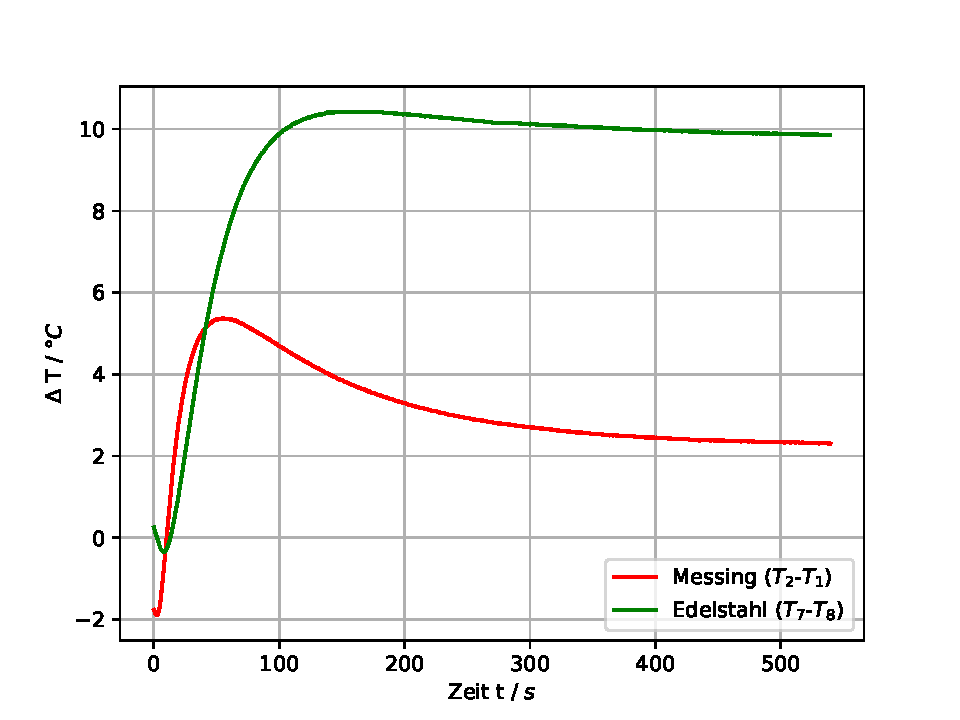
\includegraphics{Differenz.pdf}
    \caption{Temperaturdifferenzen von Messing und Edelstahl.}
    \label{fig:c}
\end{figure}

\subsection{Dynamische Methode}
Durch die dynamische Methode kann die Wärmeleitfähigkeit \kappa von verschiedenen Materialien bestimmt werden.
Bei einer periodischen Erwärmung von $\SI{80}{s}$ werden die Messwerte aufgenommen.
Nach (6) werden die Amplituden aus Abbildung (4) abgelesen und \kappa berechnet.
Aus den berechneten Werten wird dann der Mittelwert mit folgender Formel gebildet.
\begin{equation}
    \overline{x} = \frac{1}{N} \sum_{i=1}^N x_i
\end{equation}
Der dazugehörige Fehler wird folgendermaßen bestimmt.
\begin{equation}
    \Delta \overline{x} = \sqrt{\frac{1}{N(N-1)}\sum \limits_{i=1}^N (x_i-\overline{x})^2}
\end{equation}

\begin{table}[H]
    \begin{center}
      \caption{Dynamische Messmethode Messing.}
      \label{tab:c}
      \begin{tabular}{c|c|c|c} 
        \textbf{$A_\text{fern} / K$ } &  \textbf{$A_\text{nah} / K$} & \textbf{$\Delta t / s$} & \textbf{$\kappa / \frac{W}{m \cdot K}$}\\
        \hline
        11,5 &4,0 &16 & 87,359 \\
        11,0 &3,0 &17 & 94,673 \\
        11,0 &3,0 &14 & 81,149 \\
        12,0 &3,5 &10 & 119,799 \\
        11,0 &3,0 &13 & 87,391 \\
        11,5 &3,5 &12 & 103,404 \\
        10,5 &3,5 &13 & 103,353 \\
        11,0 &4,0 &12 & 121,597 \\
        11,0 &3,5 &11 & 117,183 \\
        10,0 &3,0 &12 & 102,168 \\
      \end{tabular}
    \end{center}
\end{table}

\begin{figure}[H]
    \centering
    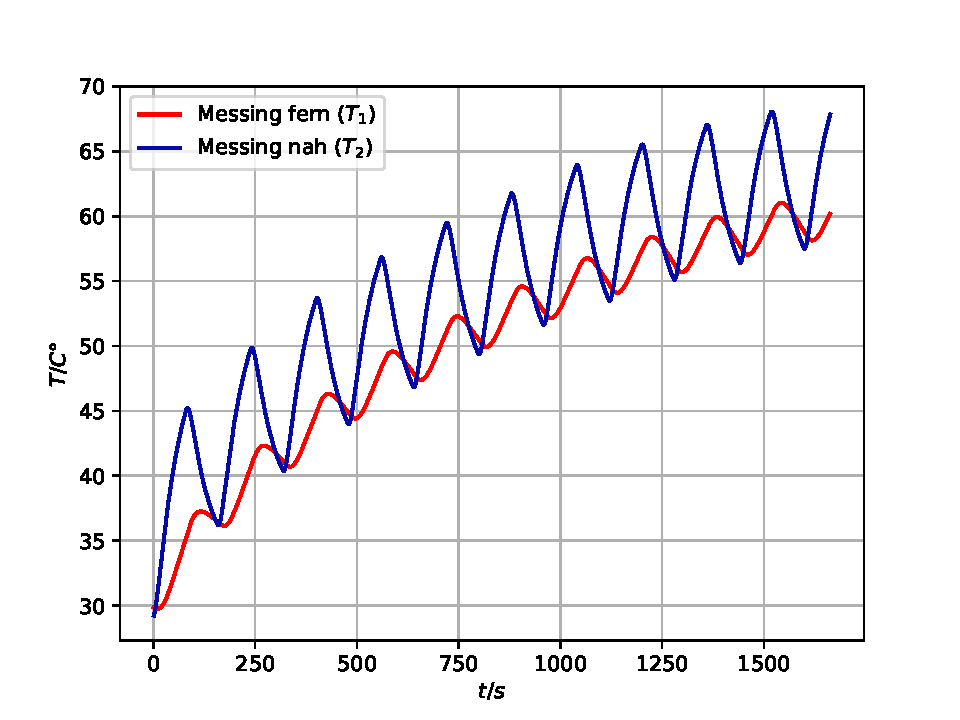
\includegraphics{Dynamisch1.pdf}
    \caption{Dynamische Methode Messing.}
    \label{fig:d}
\end{figure}

Mit diesen Werte und den Gleichungen (6),(8) und (9) ergibt sich für die Wärmeleitfähigkeit von Messing folgender Wert.
\begin{equation}
    \overline{\kappa}_\text{Messing} =  \SI{101,808 \pm 4,535}{\frac{W}{\metre\cdot\kelvin}} \notag
\end{equation}


Diese Messung wird jetzt für Aluminium ausgewertet, wobei die Werte aus Tabelle \ref{tab:d} gemessen werden.
Daraus ergibt sich die Abbildung \ref{fig:e}.
Nach Gleichung (6),(8) und (9) ergibt sich dann folgender Wert für die Wärmeleitfähigkeit von Aluminium.
\begin{equation}
    \overline{\kappa}_\text{Aluminium} =  \SI{176,969 \pm 7,631}{\frac{W}{\metre\cdot \kelvin}} \notag
\end{equation}

\begin{table}[H]
    \begin{center}
      \caption{Dynamische Messmethode Aluminium.}
      \label{tab:d}
      \begin{tabular}{c|c|c|c|c} 
        \textbf{$A_\text{fern} / K$ } &  \textbf{$A_\text{nah} / K$} & \textbf{$\Delta t / s$}& \textbf{$\Delta t / s$} & \textbf{$\kappa / \frac{W}{m \cdot K}$}\\
        \hline
        14,0 &6,5 &9 & 151,449 \\
        13,0 &5,5 &7 & 173,680 \\
        13,5 &6,0 &8 & 161,204 \\
        14,5 &5,0 &8 & 163,706 \\
        13,0 &6,5 &9 & 167,641 \\
        12,5 &6,0 &10 & 203,551 \\
        13,0 &5,0 &7 & 156,356 \\
        12,5 &4,5 &9 & 170,606 \\
        12,5 &5,0 &8&  228,268 \\
        13,0 &6,0 &14& 193,226 \\
      \end{tabular}
    \end{center}
\end{table}

\begin{figure}[H]
    \centering
    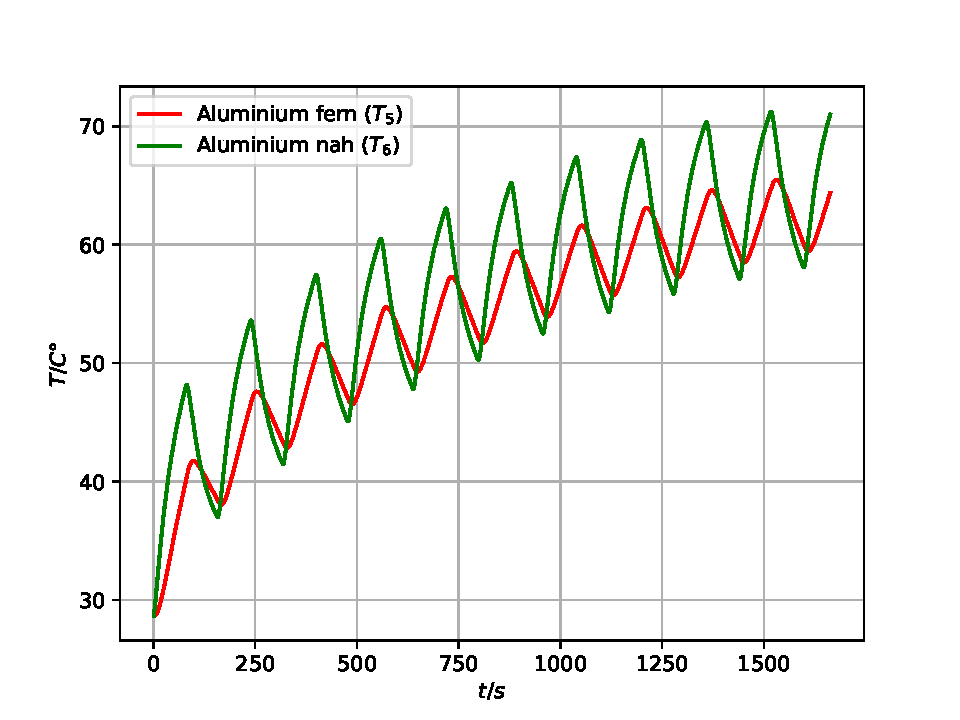
\includegraphics{Dynamisch2.pdf}
    \caption{Dynamische Methode Aluminium.}
    \label{fig:e}
\end{figure}

Die dynamische Methode wird nun mit einer Periodendauer von $\SI{200}{s}$ durchgeführt.
Es wird die Wärmeleitfähigkeit von Edelstahl experimentell bestimmt.
Das Diagramm trägit die gemessene Temperatur des fernen und nahen Thermoelements gegen die Zeit auf.
 
Durch die in Tabelle \ref{tab:e} aufgetragenen Werte und nach Gleichung (6), (8) und (9) wird nun die Wärmeleitfähigkeit von Edelstahl bestimmt.
Es ergibt sich folgender Wert.
\begin{equation}
    \overline{\kappa}_\text{Edelstahl} =  \SI{14,207 \pm 0,221}{\frac{W}{\metre\cdot \kelvin}} \notag
\end{equation}

\begin{table}[H]
    \begin{center}
      \caption{Dynamische Messmethode Edelstahl.}
      \label{tab:e}
      \begin{tabular}{c|c|c|c} 
        \textbf{$A_\text{fern} / K$ } &  \textbf{$A_\text{nah} / K$} & \textbf{$\Delta t / s$} & \textbf{$\kappa / \frac{W}{m \cdot K}$}\\
        \hline
        16,5 &2,5 &52 & 14,675 \\
        15,0 &2,0 &49 & 14,585 \\
        16,0 &2,0 &59 & 11,737 \\
        15,5 &2,5 &56 & 14,094 \\
        17,5 &1,5 &47 & 12,471 \\
        16,5 &2,0 &50 & 13,648 \\
        16,0 &1,5 &42 & 14,484 \\
        16,5 &2,0 &51 & 13,380 \\
        15,5 &2,5 &42 & 18,791 \\
      \end{tabular}
    \end{center}
\end{table}

\begin{figure}[H]
    \centering
    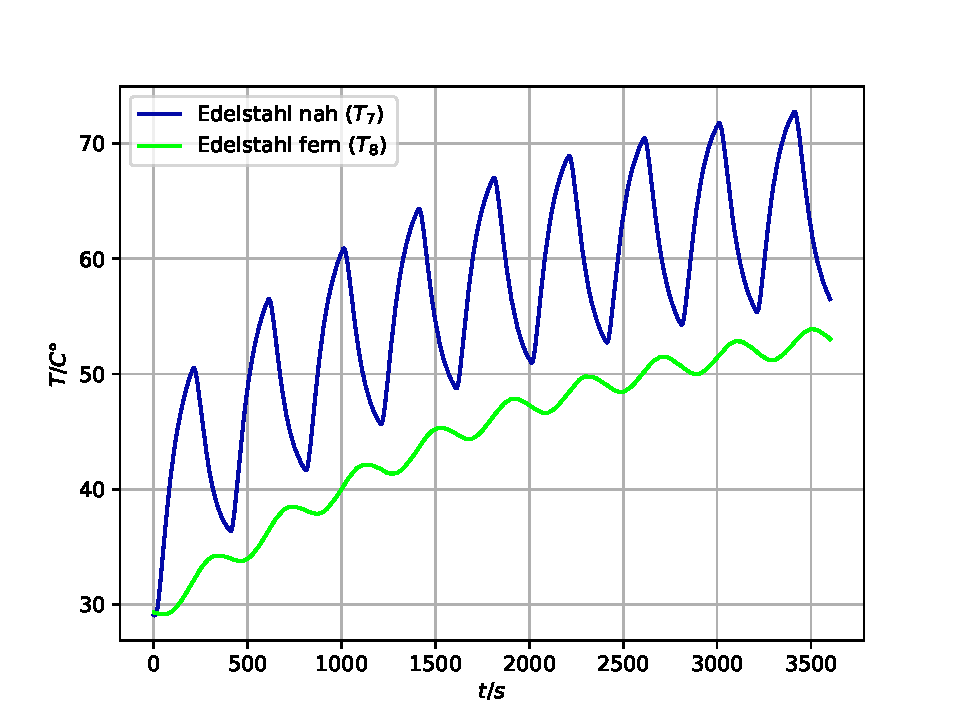
\includegraphics{Dynamisch3.pdf}
    \caption{Dynamische Methode Edelstahl.}
    \label{fig:e}
\end{figure}

Des Weiteren wird die Wellenlänge der verschiedenen Temperaturwellen nach Gleichung (5) und den Zusammenhängen $\omega = \frac{2 \pi}{T}$, $f =\frac{1}{T}$ und $v = \lambda \cdot f$ bestimmt.
Es folgt für die Wellenlänge
\begin{equation}
    \lambda = \sqrt{\frac{4 \pi \kappa T}{\rho c}}
\end{equation}.
Es ergibt sich mit der Periodendauer der beiden Methoden für die verschiedenen Materialien
\begin{equation*}
    \lambda_\text{Messing} = \SI{0,248 \pm 0,006}{\metre}
    \lambda_\text{Aluminium} = \SI{0,426 \pm 0,010}{\metre}
    \lambda_\text{Edelstahl} = \SI{0,123 \pm 0004}{\metre}
\end{equation*}.
